\documentclass[aps,pre,twocolumn,superscriptaddress,nofootinbib,10pt]{revtex4-2}
\usepackage{graphicx}
\usepackage{amsmath,amssymb}
\usepackage{url}\usepackage{xurl}


\newcommand{\nModels}{33}
\newcommand{\nRecords}{17}
\newcommand{\nNonRecords}{16}
\newcommand{\spanYears}{6.78}
\newcommand{\linSlope}{1.76}
\newcommand{\linDbl}{208}
\newcommand{\betaAll}{+0.138}
\newcommand{\hcT}{2.69}
\newcommand{\olsT}{2.90}
\newcommand{\hcPup}{0.0058}
\newcommand{\hcPdn}{0.99}
\newcommand{\olsPup}{0.0035}
\newcommand{\wildPup}{0.022}
\newcommand{\permPup}{0.0027}
\newcommand{\wildOverHc}{3.8}
\newcommand{\hcCiLo}{+0.033}
\newcommand{\hcCiHi}{+0.244}
\newcommand{\hcSe}{0.052}
\newcommand{\rrEqAll}{3.3}
\newcommand{\rateStart}{0.71}
\newcommand{\rateEnd}{2.59}
\newcommand{\dblStart}{515}
\newcommand{\dblEnd}{141}
\newcommand{\rrHat}{3.6}
\newcommand{\pbDraws}{19{,}999}
\newcommand{\realSotaBeta}{+0.114}
\newcommand{\realSotaNull}{+0.062}
\newcommand{\realMirBeta}{+0.177}
\newcommand{\realMirNull}{+0.042}
\newcommand{\realHeckBeta}{+0.054}
\newcommand{\realHeckNull}{+0.004}
\newcommand{\realIpwBeta}{+0.120}
\newcommand{\realIpwNull}{+0.053}
\newcommand{\realAuditBeta}{+0.192}
\newcommand{\realAuditNull}{+0.001}
\newcommand{\realContrBeta}{$-$0.024}
\newcommand{\realContrNull}{+0.062}
\newcommand{\realThrBeta}{+0.004}
\newcommand{\realThrNull}{+0.011}
\newcommand{\realSotaPup}{0.24}
\newcommand{\realSotaPdn}{0.76}
\newcommand{\realMirPup}{0.015}
\newcommand{\realMirPdn}{0.99}
\newcommand{\realHeckPup}{0.21}
\newcommand{\realHeckPdn}{0.79}
\newcommand{\realIpwPup}{0.20}
\newcommand{\realIpwPdn}{0.80}
\newcommand{\realAuditPup}{0.0063}
\newcommand{\realAuditPdn}{0.99}
\newcommand{\realRratePup}{0.0042}
\newcommand{\realRratePdn}{1.00}
\newcommand{\realGapPup}{0.11}
\newcommand{\realGapPdn}{0.89}
\newcommand{\realContrPup}{0.94}
\newcommand{\realContrPdn}{0.059}
\newcommand{\realThrPup}{0.53}
\newcommand{\realThrPdn}{0.47}
\newcommand{\realGapObs}{$-$0.87}
\newcommand{\realGapNull}{$-$1.36}
\newcommand{\realRrateObs}{$-$0.43}
\newcommand{\realRrateNull}{$-$1.05}
\newcommand{\realSotaRrEq}{2.6}
\newcommand{\realMirRrEq}{5.3}
\newcommand{\realHeckRrEq}{1.5}
\newcommand{\realIpwRrEq}{2.7}
\newcommand{\realAuditRrEq}{6.7}
\newcommand{\auditMed}{+0.128}
\newcommand{\auditQlo}{0.095}
\newcommand{\auditQhi}{0.177}
\newcommand{\auditMin}{0.019}
\newcommand{\auditMax}{0.252}
\newcommand{\mbAllLo}{+0.045}
\newcommand{\mbAllHi}{+0.629}
\newcommand{\mbSotaLo}{+0.002}
\newcommand{\mbSotaHi}{+0.440}
\newcommand{\mbHeckLo}{$-$0.044}
\newcommand{\mbHeckHi}{+0.455}
\newcommand{\mbAuditLo}{$-$0.019}
\newcommand{\mbAuditHi}{+0.644}
\newcommand{\mbDraws}{2{,}000}
\newcommand{\mbAllRrEqLo}{1.4}
\newcommand{\rrHatLo}{1.3}
\newcommand{\rrHatHi}{17.5}
\newcommand{\rrHatMed}{3.2}
\newcommand{\rrHatNonpos}{50}
\newcommand{\loroMax}{0.030}
\newcommand{\loroSd}{0.039}
\newcommand{\preregReal}{\texttt{17d741c}}
\newcommand{\numpyV}{2.5.5}
\newcommand{\scipyV}{1.18.1}
\newcommand{\runsSha}{\texttt{f489d11728909937\ldots}}
\newcommand{\lastHorizonH}{4.1}
\newcommand{\holmHc}{0.029}
\newcommand{\holmAudit}{0.029}
\newcommand{\holmHeck}{0.63}
\newcommand{\holmRrate}{0.025}
\newcommand{\holmContr}{1}
\newcommand{\holmThr}{1}
\newcommand{\hbCiLo}{$-$0.044}
\newcommand{\hbCiHi}{+0.244}
\newcommand{\iidFp}{0.0009}
\newcommand{\origIid}{27.9}
\newcommand{\origIidLo}{25.1}
\newcommand{\origIidHi}{30.8}
\newcommand{\origIidK}{279}
\newcommand{\origIidN}{1{,}000}
\newcommand{\origHb}{35.4}
\newcommand{\origHbLo}{32.4}
\newcommand{\origHbHi}{38.5}
\newcommand{\origHbK}{354}
\newcommand{\origHbN}{1{,}000}
\newcommand{\origIidAll}{8.7}
\newcommand{\origIidAllLo}{7.0}
\newcommand{\origIidAllHi}{10.6}
\newcommand{\origIidAllK}{87}
\newcommand{\origIidAllN}{1{,}000}
\newcommand{\origHbAll}{23.9}
\newcommand{\origHbAllLo}{21.3}
\newcommand{\origHbAllHi}{26.7}
\newcommand{\origHbAllK}{239}
\newcommand{\origHbAllN}{1{,}000}
\newcommand{\origMeanRecords}{11.3}
\newcommand{\sigmaM}{0.94}
\newcommand{\sigmaJ}{1.67}
\newcommand{\phiFam}{0.64}
\newcommand{\simAZero}{$-$5.23}
\newcommand{\rateNull}{1.74}
\newcommand{\dblNull}{210}
\newcommand{\simValN}{200}
\newcommand{\biasSota}{0.0706}
\newcommand{\biasRrSota}{1.76}
\newcommand{\biasSeSota}{0.0005}
\newcommand{\biasMir}{0.0504}
\newcommand{\biasRrMir}{1.49}
\newcommand{\biasSeMir}{0.0004}
\newcommand{\biasHeck}{0.0092}
\newcommand{\biasRrHeck}{1.07}
\newcommand{\biasSeHeck}{0.0004}
\newcommand{\biasIpw}{0.0617}
\newcommand{\biasRrIpw}{1.63}
\newcommand{\biasSeIpw}{0.0005}
\newcommand{\biasAudit}{0.0023}
\newcommand{\biasRrAudit}{1.02}
\newcommand{\biasSeAudit}{0.0004}
\newcommand{\biasAll}{0.0021}
\newcommand{\biasRrAll}{1.02}
\newcommand{\biasSeAll}{0.0003}
\newcommand{\sizeCclUp}{11.8}
\newcommand{\sizeCclTwo}{12.2}
\newcommand{\sizeCclUpN}{16.0}
\newcommand{\sizeTclUp}{20.7}
\newcommand{\sizeTclTwo}{18.9}
\newcommand{\sizeTclUpN}{19.6}
\newcommand{\sizeMirUp}{6.2}
\newcommand{\sizeMirTwo}{7.0}
\newcommand{\sizeMirUpN}{11.2}
\newcommand{\sizeHeckUp}{6.6}
\newcommand{\sizeHeckTwo}{6.4}
\newcommand{\sizeHeckUpN}{10.5}
\newcommand{\sizeIpwUp}{5.7}
\newcommand{\sizeIpwTwo}{6.2}
\newcommand{\sizeIpwUpN}{8.1}
\newcommand{\sizeAuditUp}{6.0}
\newcommand{\sizeAuditTwo}{6.2}
\newcommand{\sizeAuditUpN}{9.1}
\newcommand{\sizeRrateUp}{4.7}
\newcommand{\sizeRrateTwo}{4.5}
\newcommand{\sizeRrateUpN}{5.1}
\newcommand{\sizeGapUp}{5.3}
\newcommand{\sizeGapTwo}{5.1}
\newcommand{\sizeGapUpN}{7.8}
\newcommand{\sizeContrUp}{5.4}
\newcommand{\sizeContrTwo}{4.9}
\newcommand{\sizeContrUpN}{5.0}
\newcommand{\sizeThrUp}{5.5}
\newcommand{\sizeThrTwo}{5.0}
\newcommand{\sizeThrUpN}{6.0}
\newcommand{\sizeSotaUp}{5.9}
\newcommand{\sizeSotaTwo}{6.6}
\newcommand{\sizeSotaUpN}{9.1}
\newcommand{\sizeAuditUpLo}{5.8}
\newcommand{\sizeAuditUpHi}{6.3}
\newcommand{\sizeHeckUpLo}{6.4}
\newcommand{\sizeHeckUpHi}{6.9}
\newcommand{\nRobust}{3}
\newcommand{\nSizeValid}{6}
\newcommand{\nMethods}{10}
\newcommand{\robustMin}{4.2}
\newcommand{\robustMax}{6.0}
\newcommand{\dblStartRrA}{236}
\newcommand{\dblEndRrA}{189}
\newcommand{\dblStartRrB}{262}
\newcommand{\dblEndRrB}{175}
\newcommand{\dblStartRrTwo}{315}
\newcommand{\dblEndRrTwo}{158}
\newcommand{\dblStartRrThree}{420}
\newcommand{\dblEndRrThree}{140}
\newcommand{\dblStartRrFour}{525}
\newcommand{\dblEndRrFour}{131}
\newcommand{\dblStartRrTwoOld}{304}
\newcommand{\dblEndRrTwoOld}{160}
\newcommand{\dblStartRrFourOld}{473}
\newcommand{\dblEndRrFourOld}{135}
\newcommand{\rrTwoOldRatio}{1.90}
\newcommand{\rrFourOldRatio}{3.50}
\newcommand{\decAudit}{63.5}
\newcommand{\decHeck}{33.3}
\newcommand{\decSota}{36.2}
\newcommand{\decRrate}{19.5}
\newcommand{\powCclTwo}{27.9}
\newcommand{\powCclThree}{49.1}
\newcommand{\powCclFour}{61.4}
\newcommand{\rawpowCclTwo}{46.4}
\newcommand{\powTclTwo}{13.4}
\newcommand{\powTclThree}{19.0}
\newcommand{\powTclFour}{22.6}
\newcommand{\rawpowTclTwo}{43.1}
\newcommand{\powMirTwo}{27.6}
\newcommand{\powMirThree}{48.1}
\newcommand{\powMirFour}{59.7}
\newcommand{\rawpowMirTwo}{32.6}
\newcommand{\powHeckTwo}{19.4}
\newcommand{\powHeckThree}{32.9}
\newcommand{\powHeckFour}{41.9}
\newcommand{\rawpowHeckTwo}{25.2}
\newcommand{\powIpwTwo}{15.0}
\newcommand{\powIpwThree}{23.6}
\newcommand{\powIpwFour}{29.9}
\newcommand{\rawpowIpwTwo}{17.7}
\newcommand{\powAuditTwo}{24.5}
\newcommand{\powAuditThree}{41.6}
\newcommand{\powAuditFour}{52.8}
\newcommand{\rawpowAuditTwo}{27.5}
\newcommand{\powRrateTwo}{13.4}
\newcommand{\powRrateThree}{20.9}
\newcommand{\powRrateFour}{27.0}
\newcommand{\rawpowRrateTwo}{13.2}
\newcommand{\powGapTwo}{13.0}
\newcommand{\powGapThree}{19.2}
\newcommand{\powGapFour}{22.2}
\newcommand{\rawpowGapTwo}{13.6}
\newcommand{\powContrTwo}{2.9}
\newcommand{\powContrThree}{1.7}
\newcommand{\powContrFour}{1.2}
\newcommand{\rawpowContrTwo}{3.2}
\newcommand{\powThrTwo}{4.0}
\newcommand{\powThrThree}{3.2}
\newcommand{\powThrFour}{3.2}
\newcommand{\rawpowThrTwo}{4.7}
\newcommand{\powSotaTwo}{17.9}
\newcommand{\powSotaThree}{30.2}
\newcommand{\powSotaFour}{38.3}
\newcommand{\rawpowSotaTwo}{21.6}
\newcommand{\powMaxTwo}{27.9}
\newcommand{\powMaxThree}{49.1}
\newcommand{\powMaxFour}{61.4}
\newcommand{\powCap}{28}
\newcommand{\loroAuc}{0.51}
\newcommand{\loroAucLo}{0.49}
\newcommand{\loroAucHi}{0.52}
\newcommand{\aThreeReps}{270{,}000}
\newcommand{\aThreeCells}{17}
\newcommand{\preregAThree}{\texttt{03dfe34}}
\newcommand{\triA}{18}
\newcommand{\triB}{117}
\newcommand{\triC}{33}
\newcommand{\triD}{72}
\newcommand{\triN}{240}
\newcommand{\baseMbSota}{5.2}
\newcommand{\baseMbSotaHalf}{7.8}
\newcommand{\baseMbSotaQuarter}{12.3}
\newcommand{\baseMbAll}{4.1}
\newcommand{\baseMbAllHalf}{8.2}
\newcommand{\baseMbAllQuarter}{14.6}
\newcommand{\basePbSota}{6.5}
\newcommand{\basePbSotaHalf}{12.6}
\newcommand{\basePbSotaQuarter}{24.5}
\newcommand{\baseIidAll}{8.2}
\newcommand{\baseIidAllHalf}{17.9}
\newcommand{\baseIidAllQuarter}{33.4}
\newcommand{\baseHbAll}{22.9}
\newcommand{\baseHbAllHalf}{8.0}
\newcommand{\baseHbAllQuarter}{3.4}
\newcommand{\baseIidSota}{26.3}
\newcommand{\baseIidSotaHalf}{32.1}
\newcommand{\baseIidSotaQuarter}{40.1}
\newcommand{\baseHbSota}{37.7}
\newcommand{\baseHbSotaHalf}{17.9}
\newcommand{\baseHbSotaQuarter}{6.6}
\newcommand{\baseXbAll}{1.4}
\newcommand{\baseXbAllHalf}{0.5}
\newcommand{\baseXbAllQuarter}{0.4}
\newcommand{\baseXbSota}{1.7}
\newcommand{\baseXbSotaHalf}{1.0}
\newcommand{\baseXbSotaQuarter}{0.4}
\newcommand{\baseN}{3{,}000}
\newcommand{\baseMeanRecords}{11.2}
\newcommand{\baseMbSotaEven}{9.2}
\newcommand{\baseIidAllPowTwo}{30}
\newcommand{\baseIidAllRawTwo}{34.8}
\newcommand{\baseNNoise}{2{,}100}
\newcommand{\baseNEven}{3{,}000}
\newcommand{\illBias}{0.064}
\newcommand{\illRr}{1.67}
\newcommand{\illRecords}{11.3}
\newcommand{\illReps}{40{,}000}
\newcommand{\holdN}{3}
\newcommand{\holdInside}{3}
\newcommand{\holdAbove}{3}
\newcommand{\holdHbLo}{+0.27}
\newcommand{\holdHbHi}{+1.17}
\newcommand{\uInside}{35}
\newcommand{\uN}{40}
\newcommand{\uCov}{87.5}
\newcommand{\uCbLo}{67}
\newcommand{\uCbHi}{100}
\newcommand{\uSeries}{4}
\newcommand{\uInsideEighty}{26}
\newcommand{\uCovEighty}{65}
\newcommand{\uMetrInside}{0}
\newcommand{\uMetrN}{2}
\newcommand{\holmWild}{0.088}
\newcommand{\uGap}{21}
\newcommand{\auditDrawAbove}{above}
\newcommand{\typeMAuditB}{3.5}
\newcommand{\typeMAllB}{2.3}
\newcommand{\typeMSotaB}{4.8}
\newcommand{\typeMHeckB}{3.1}
\newcommand{\typeMAuditTwo}{2.2}
\newcommand{\typeMAllTwo}{1.6}
\newcommand{\typeMSotaTwo}{3.0}
\newcommand{\typeMHeckTwo}{1.9}
\newcommand{\typeMAuditThree}{1.6}
\newcommand{\typeMAllThree}{1.3}
\newcommand{\typeMSotaThree}{2.1}
\newcommand{\typeMHeckThree}{1.4}
\newcommand{\typeMAuditFour}{1.4}
\newcommand{\typeMAllFour}{1.2}
\newcommand{\typeMSotaFour}{1.8}
\newcommand{\typeMHeckFour}{1.2}
\newcommand{\trueBetaTwo}{0.086}
\newcommand{\typeMAllGivenTwo}{+0.138}
\newcommand{\typeMAuditGivenTwo}{+0.188}
\newcommand{\typeMAllGivenNull}{+0.084}
\newcommand{\typeMAuditGivenNull}{+0.171}
\newcommand{\looMin}{+0.116}
\newcommand{\looMax}{+0.167}
\newcommand{\looPmax}{0.099}
\newcommand{\looNsig}{31}
\newcommand{\looPGptTwo}{0.056}
\newcommand{\looBGptTwo}{+0.160}
\newcommand{\looPGptThree}{0.099}
\newcommand{\looBGptThree}{+0.138}
\newcommand{\dropPreTwentyThreeN}{30}
\newcommand{\dropPreTwentyThreeBeta}{+0.676}
\newcommand{\dropPreTwentyThreeP}{0.030}
\newcommand{\dropPreTwentyThreeWild}{0.080}
\newcommand{\dropFirstTwoN}{31}
\newcommand{\dropFirstTwoBeta}{+0.232}
\newcommand{\dropFirstTwoP}{0.31}
\newcommand{\dropFirstTwoWild}{0.083}
\newcommand{\auditManyN}{20{,}000}
\newcommand{\auditManyMean}{+0.137}
\newcommand{\auditManyMed}{+0.134}
\newcommand{\auditManyQlo}{0.102}
\newcommand{\auditManyQhi}{0.171}
\newcommand{\auditManyShare}{85}
\newcommand{\schedRealRr}{1.67}
\newcommand{\schedRealBeta}{+0.064}
\newcommand{\schedEvenRr}{0.86}
\newcommand{\schedEvenBeta}{$-$0.019}
\newcommand{\schedReflRr}{0.82}
\newcommand{\schedReflBeta}{$-$0.025}
\newcommand{\pvMin}{0.0027}
\newcommand{\pvMax}{0.022}
\newcommand{\preregATwo}{\texttt{8c66022}}
\newcommand{\aTwoOlsUp}{6.8}
\newcommand{\aTwoOlsTwo}{8.1}
\newcommand{\aTwoHcUp}{5.1}
\newcommand{\aTwoHcTwo}{5.1}
\newcommand{\aTwoWildUp}{4.8}
\newcommand{\aTwoWildTwo}{4.6}
\newcommand{\aTwoPermUp}{6.7}
\newcommand{\aTwoPermTwo}{7.9}
\newcommand{\aTwoMbAllUp}{4.5}
\newcommand{\aTwoMbAllTwo}{3.9}
\newcommand{\aTwoMbSotaUp}{13.7}
\newcommand{\aTwoMbSotaTwo}{5.8}
\newcommand{\aTwoPbSotaUp}{5.9}
\newcommand{\aTwoPbSotaTwo}{6.6}
\newcommand{\aTwoHcUpLo}{4.9}
\newcommand{\aTwoHcUpHi}{5.3}
\newcommand{\aTwoHcUpE}{8.3}
\newcommand{\aTwoHcTwoE}{8.5}
\newcommand{\aTwoHcUpKfour}{0.6}
\newcommand{\aTwoHcTwoKfour}{12.2}
\newcommand{\aTwoHcUpNhalf}{9.3}
\newcommand{\aTwoHcTwoNhalf}{10.5}
\newcommand{\aTwoHcUpNquarter}{14.7}
\newcommand{\aTwoHcTwoNquarter}{18.9}
\newcommand{\aTwoHcDnKfour}{17.8}
\newcommand{\aTwoWildUpLo}{4.6}
\newcommand{\aTwoWildUpHi}{5.0}
\newcommand{\aTwoWildUpE}{8.8}
\newcommand{\aTwoWildTwoE}{9.1}
\newcommand{\aTwoWildUpKfour}{0.7}
\newcommand{\aTwoWildTwoKfour}{11.6}
\newcommand{\aTwoWildUpNhalf}{8.4}
\newcommand{\aTwoWildTwoNhalf}{9.4}
\newcommand{\aTwoWildUpNquarter}{13.6}
\newcommand{\aTwoWildTwoNquarter}{19.1}
\newcommand{\aTwoWildDnKfour}{19.9}
\newcommand{\aTwoMbSotaUpX}{13.68}
\newcommand{\aTwoMbSotaTwoX}{5.85}
\newcommand{\aTwoMbSotaDnX}{0.37}
\newcommand{\aTwoPowOlsA}{11.8}
\newcommand{\aTwoPowOlsB}{20.9}
\newcommand{\aTwoPowOlsTwo}{40.2}
\newcommand{\aTwoPowOlsThree}{67.6}
\newcommand{\aTwoPowOlsFour}{80.8}
\newcommand{\aTwoRawOlsTwo}{46.8}
\newcommand{\aTwoPowHcA}{10.7}
\newcommand{\aTwoPowHcB}{18.5}
\newcommand{\aTwoPowHcTwo}{34.0}
\newcommand{\aTwoPowHcThree}{56.7}
\newcommand{\aTwoPowHcFour}{68.5}
\newcommand{\aTwoRawHcTwo}{34.7}
\newcommand{\aTwoPowWildA}{10.7}
\newcommand{\aTwoPowWildB}{18.5}
\newcommand{\aTwoPowWildTwo}{34.0}
\newcommand{\aTwoPowWildThree}{56.7}
\newcommand{\aTwoPowWildFour}{68.5}
\newcommand{\aTwoRawWildTwo}{33.0}
\newcommand{\aTwoPowPermA}{11.8}
\newcommand{\aTwoPowPermB}{20.9}
\newcommand{\aTwoPowPermTwo}{40.2}
\newcommand{\aTwoPowPermThree}{67.6}
\newcommand{\aTwoPowPermFour}{80.8}
\newcommand{\aTwoRawPermTwo}{46.1}
\newcommand{\aTwoPowMbAllA}{10.0}
\newcommand{\aTwoPowMbAllB}{16.5}
\newcommand{\aTwoPowMbAllTwo}{29.4}
\newcommand{\aTwoPowMbAllThree}{46.8}
\newcommand{\aTwoPowMbAllFour}{57.2}
\newcommand{\aTwoRawMbAllTwo}{27.4}
\newcommand{\aTwoPowHcTwoLo}{32.8}
\newcommand{\aTwoPowHcTwoHi}{35.1}
\newcommand{\aTwoPowWildTwoLo}{32.7}
\newcommand{\aTwoPowWildTwoHi}{35.2}
\newcommand{\aTwoPowHcTwoRound}{34}
\newcommand{\aTwoValHc}{4.9}
\newcommand{\aTwoValOls}{4.8}
\newcommand{\aTwoPairWildHc}{$-$1.67}
\newcommand{\ladZeroAll}{$-$0.0004}
\newcommand{\ladZeroSe}{0.0004}
\newcommand{\ladZeroRecRr}{1.66}
\newcommand{\ladOneAll}{+0.0025}
\newcommand{\ladOneSe}{0.0004}
\newcommand{\ladOneRecRr}{1.73}
\newcommand{\ladRecRrMin}{1.58}
\newcommand{\ladRecRrMax}{1.73}
\newcommand{\ladAllMin}{$-$0.0060}
\newcommand{\ladAllMax}{+0.0025}
\newcommand{\ladHcMin}{3.4}
\newcommand{\ladHcMax}{4.1}
\newcommand{\ladOlsMin}{4.8}
\newcommand{\ladOlsMax}{5.7}
\newcommand{\ladMbSotaMin}{11.1}
\newcommand{\ladMbSotaMax}{12.2}
\newcommand{\ladOlsTwoBefore}{4.8}
\newcommand{\ladOlsTwoAfter}{8.0}
\newcommand{\aTwoKfourAll}{$-$0.051}
\newcommand{\aTwoKfourCeil}{20}
\newcommand{\aTwoRAll}{+0.0021}
\newcommand{\aTwoRAllSe}{0.0003}
\newcommand{\aTwoReps}{676{,}900}
\newcommand{\clG}{7}
\newcommand{\clMax}{15}
\newcommand{\clSingles}{3}
\newcommand{\clSecond}{9}
\newcommand{\clT}{1.99}
\newcommand{\clDf}{1.5}
\newcommand{\clP}{0.112}
\newcommand{\clPtwo}{0.224}
\newcommand{\clWebb}{0.094}
\newcommand{\clWebbTwo}{0.188}
\newcommand{\clRad}{0.086}
\newcommand{\clTDrop}{1.31}
\newcommand{\clDfDrop}{1.8}
\newcommand{\clPDrop}{0.168}
\newcommand{\clPtwoDrop}{0.336}
\newcommand{\clWebbDrop}{0.060}
\newcommand{\clWebbTwoDrop}{0.121}
\newcommand{\clRadDrop}{0.062}
\newcommand{\clWebbB}{99{,}999}
\newcommand{\clRadN}{128}
\newcommand{\clNullQ}{2.55}
\newcommand{\cfPass}{2}
\newcommand{\cfSign}{7}
\newcommand{\cfN}{8}
\newcommand{\cfReps}{40{,}000}
\newcommand{\cfReal}{+0.057}
\newcommand{\cfRealSim}{+0.064}
\newcommand{\cfRealErr}{11}
\newcommand{\cfEven}{$-$0.024}
\newcommand{\cfEvenSim}{$-$0.019}
\newcommand{\cfEvenErr}{30}
\newcommand{\cfRefl}{$-$0.029}
\newcommand{\cfReflSim}{$-$0.025}
\newcommand{\cfReflErr}{18}
\newcommand{\cfRecErr}{0.13}
\newcommand{\cfErrMin}{17}
\newcommand{\cfErrMax}{102}
\newcommand{\cfRealRr}{1.66}
\newcommand{\cfEvenRr}{0.86}
\newcommand{\cfReflRr}{0.82}
\newcommand{\cfNeg}{6}
\newcommand{\cfOther}{7}
\newcommand{\csReps}{4{,}000}
\newcommand{\csWebbB}{999}
\newcommand{\csCells}{6}
\newcommand{\csWebbValid}{5}
\newcommand{\csCrValid}{1}
\newcommand{\csCrCons}{3}
\newcommand{\csRadValid}{4}
\newcommand{\csWebbMin}{3.7}
\newcommand{\csWebbMax}{5.5}
\newcommand{\csCrMin}{2.2}
\newcommand{\csCrMax}{5.1}
\newcommand{\csCrLowMax}{3.4}
\newcommand{\csWebbGauss}{3.7}
\newcommand{\csWebbGaussLo}{3.2}
\newcommand{\csWebbGaussHi}{4.4}
\newcommand{\csWebbDevA}{4.8}
\newcommand{\csWebbDevB}{4.5}
\newcommand{\csCrDevA}{2.7}
\newcommand{\csCrDevB}{2.2}
\newcommand{\mbN}{22}
\newcommand{\mbBarOne}{18}
\newcommand{\mbBarTwo}{9}
\newcommand{\mbOver}{9}
\newcommand{\mbOverPct}{41}
\newcommand{\mbMid}{4}
\newcommand{\mbCovPlus}{0.80}
\newcommand{\mbCovMinus}{0.91}
\newcommand{\mbRelBias}{9.3}
\newcommand{\mbRefSize}{4.7}
\newcommand{\mbCheckIid}{4.9}
\newcommand{\mbClUnmeasured}{2}
\newcommand{\mbIidMin}{5.3}
\newcommand{\mbIidMax}{32.3}
\newcommand{\mbMbMin}{1.8}
\newcommand{\mbMbMax}{38.1}
\newcommand{\mbOverMin}{13}
\newcommand{\mbOverMax}{66}
\newcommand{\mbPowPlusMax}{5.5}
\newcommand{\mbPowMinusMax}{34}
\newcommand{\mbMetrEpoch}{3.7}
\newcommand{\mbExcluded}{69}
\newcommand{\mbRhoM}{0.27}
\newcommand{\mbRhoMP}{0.22}
\newcommand{\mbRhoRec}{0.29}
\newcommand{\mbRhoRecP}{0.19}
\newcommand{\mbNNoMetr}{21}
\newcommand{\mbBarOneNoMetr}{17}
\newcommand{\mbOverNoMetr}{9}
\newcommand{\mbBarTwoNoMetr}{9}
\newcommand{\mbBiasNeg}{20}
\newcommand{\mbBiasNegSign}{20}
\newcommand{\mbRepBelowMed}{8405}
\newcommand{\mbRepNegMed}{78}
\newcommand{\mbClN}{20}
\newcommand{\mbClOver}{5}
\newcommand{\mbMmin}{38}
\newcommand{\mbMmax}{204}
\newcommand{\mbRecMin}{8}
\newcommand{\mbRecMax}{23}
\newcommand{\mbIidValidMin}{568}
\newcommand{\mbMbValidMin}{845}
\newcommand{\mbIidOneOver}{3}
\newcommand{\mbIidOneCons}{11}
\newcommand{\mbIidOneUnder}{8}
\newcommand{\mbMbOneOver}{1}
\newcommand{\mbMbOneCons}{3}
\newcommand{\mbMbOneUnder}{18}
\newcommand{\mbMbTwoOverNull}{9}
\newcommand{\mbIidTwoOverAtt}{14}
\newcommand{\mbIidOneOverAtt}{2}
\newcommand{\mbMbTwoOverAtt}{9}
\newcommand{\mbMbOneOverAtt}{1}
\newcommand{\mbIidValidMax}{881}
\newcommand{\mbMbValidMax}{997}
\newcommand{\mbIidInvalidMaxPct}{43}
\newcommand{\mbIidOneMin}{0.9}
\newcommand{\mbIidOneMax}{26.7}
\newcommand{\mbMbOneMin}{0.0}
\newcommand{\mbMbOneMax}{11.2}
\newcommand{\mbMbOneBelowOne}{17}
\newcommand{\mbRefOne}{4.6}
\newcommand{\mbRefOneLo}{3.3}
\newcommand{\mbRefOneHi}{6.2}
\newcommand{\mbRefOneN}{875}
\newcommand{\mbRefIidOne}{25.1}
\newcommand{\mbRefIidTwo}{18.6}
\newcommand{\mbRefIidN}{657}
\newcommand{\mbRefOnePone}{2.7}
\newcommand{\rrEqPole}{0.26}
\newcommand{\rrEqMaxQ}{0.54}
\newcommand{\rrEqMax}{3.3}
\newcommand{\impN}{87}
\newcommand{\impHcast}{80}
\newcommand{\impRe}{7}
\newcommand{\impSwaa}{660}
\newcommand{\impP}{0.041}
\newcommand{\impBeta}{+0.116}
\newcommand{\impHWith}{-4.22}
\newcommand{\impHWithout}{-4.93}
\newcommand{\proxSimMin}{1.56}
\newcommand{\proxSimMax}{1.84}
\newcommand{\proxAllBeta}{+0.239}
\newcommand{\proxDropP}{0.40}
\newcommand{\proxAvailP}{0.020}
\newcommand{\proxAvailPb}{0.057}
\newcommand{\tieNameN}{17}
\newcommand{\tieRevN}{18}
\newcommand{\tieGroupN}{17}
\newcommand{\tieRandSeventeen}{43}
\newcommand{\tieRandEighteen}{57}
\newcommand{\tieSimName}{+0.0635}
\newcommand{\tieSimGroup}{+0.0643}
\newcommand{\tieSimRev}{+0.0635}
\newcommand{\tieRrName}{1.66}
\newcommand{\tieRrGroup}{1.67}
\newcommand{\levOpenAI}{72}
\newcommand{\levGptTwo}{29}
\newcommand{\levAnthropic}{18}
\newcommand{\looOpenAIP}{0.45}
\newcommand{\looOpenAIBeta}{+0.132}
\newcommand{\looAnthP}{0.031}
\newcommand{\looOpenAIRec}{$-$0.259}
\newcommand{\looOtherPMax}{0.0068}
\newcommand{\satOverMin}{2}
\newcommand{\satOverMax}{4}
\newcommand{\satRefP}{26}
\newcommand{\satRefPF}{25}
\newcommand{\proxReps}{40{,}000}
\newcommand{\hgR}{10{,}000}
\newcommand{\hgPost}{22}
\newcommand{\hgAiccDiffV}{0.06}
\newcommand{\hgAiccDiff}{0.13}
\newcommand{\hgBicDiff}{0.8}
\newcommand{\hgCvQ}{0.68}
\newcommand{\hgCvH}{0.65}
\newcommand{\hgCQ}{0.138}
\newcommand{\hgCQH}{$-$0.015}
\newcommand{\hgCQHp}{0.89}
\newcommand{\hgJointGivenC}{0.61}
\newcommand{\hgD}{+0.38}
\newcommand{\hgG}{+1.23}
\newcommand{\hgDp}{0.23}
\newcommand{\hgGp}{0.089}
\newcommand{\hgJointP}{0.24}
\newcommand{\hgTLSelL}{78.3}
\newcommand{\hgTLSelQ}{14.6}
\newcommand{\hgTLSelH}{7.1}
\newcommand{\hgTQSelL}{19.0}
\newcommand{\hgTQSelQ}{69.2}
\newcommand{\hgTQSelH}{11.8}
\newcommand{\hgTHSelL}{15.9}
\newcommand{\hgTHSelQ}{44.8}
\newcommand{\hgTHSelH}{39.4}
\newcommand{\hgPCHSelL}{0.4}
\newcommand{\hgPCHSelQ}{1.8}
\newcommand{\hgPCHSelH}{97.9}
\newcommand{\hgPCQSelL}{11.8}
\newcommand{\hgPCQSelQ}{77.1}
\newcommand{\hgPCQSelH}{11.2}
\newcommand{\stModels}{20}
\newcommand{\stSplits}{200}
\newcommand{\stDone}{$-$0.008}
\newcommand{\stDoneLo}{$-$0.14}
\newcommand{\stDoneHi}{+0.12}
\newcommand{\stDtwo}{+0.041}
\newcommand{\stDtwoLo}{$-$0.08}
\newcommand{\stDtwoHi}{+0.20}
\newcommand{\stDoneTwLo}{$-$0.17}
\newcommand{\stDoneTwHi}{+0.17}
\newcommand{\stDtwoTwLo}{$-$0.20}
\newcommand{\stDtwoTwHi}{+0.19}
\newcommand{\stCone}{+0.007}
\newcommand{\stConeSe}{0.003}
\newcommand{\stCsel}{0.66}
\newcommand{\stCrep}{0.67}
\newcommand{\stCall}{0.62}
\newcommand{\stR}{0.78}
\newcommand{\stLodoDtwoMin}{$-$0.06}
\newcommand{\stLodoDtwoMax}{+0.04}

\newcommand{\SM}{SM}
\newcommand{\rr}{rr}
\newcommand{\rreq}{rr_{\rm eq}}
\makeatletter\renewcommand\p@subsection{\thesection.}\makeatother



\begin{document}

\title{Record selection can mimic or mask acceleration in AI benchmarks}

\author{Adam Faust}
\affiliation{MOBLUEHQ, Inc., Long Grove, Illinois, USA}
\date{26 November 2026}

\begin{abstract}
An upward bend in the best-so-far curve of AI progress is read as acceleration. We ask whether it can appear with no acceleration, because a record-setting model is selected partly for favourable noise. On the release dates and design of the public METR time-horizon data (\nModels\ models, 170 tasks) we simulate exactly steady exponential progress. A quadratic fitted to the record-setting models then bends upward on average as much as a trend whose growth rate rises \biasRrSota-fold across the window; the fit through all models shows no such bias. The direction depends on the calendar: the bias was downward on \cfNeg\ of \cfOther\ alternative schedules, and when we planted a known upward bend into date-permuted scores of \mbN\ public AI benchmarks, the mean record-only curvature bent downward in \mbBiasNegSign\ of them. Standard inference neither controls false alarms nor has high power: the usual two-sided $F$ test on the records, applied to date-permuted benchmark series without a planted trend, was oversized in \mbBarOne\ of \mbN\ series (\mbIidTwoOverAtt\ of \mbN\ counting undefined fits as non-rejections), while a size-valid robust test on all models had \aTwoPowHcTwoRound\% power against a doubled growth rate. In the observed series the bend of the record curve is compatible with constant growth (one-sided $p=\realSotaPup$). The all-model curvature is positive (one-sided HC3 $p=\hcPup$, models treated as independent), but its evidence weakens when an early model is omitted, two stand-ins are redated or dropped, or developer clustering is allowed (redating raises the estimate) (Webb cluster-bootstrap $p=\clWebb$). We do not claim that AI progress is or is not accelerating. Only the first size tests of the record-only fit and the two-sided benchmark audit are confirmatory; all else is exploratory (the bias, calendar and corrected-test results were pre-registered).
\end{abstract}

\maketitle

\section{Introduction}
A much-used summary of progress in AI is the length of task, measured by the time a skilled human needs, that a model completes with 50\% reliability. Kwa \emph{et al.}\ \cite{kwa2025} estimated this ``time horizon'' for models released since 2019 and reported an exponential trend with a doubling time of roughly seven months for the frontier. Whether that trend is now steeper than exponential matters for forecasts \cite{denain2026}.

\emph{The question.} Claims about a changing pace usually rest on the best result so far, that is, on the models that set a record when they were released. A record is by definition an observation that exceeded everything before it, so it is selected partly on its noise, even when every model is measured without bias. If progress were exactly steady, would a curve fitted through the records still bend? And with a few dozen models, can any test tell steady progress from accelerating progress?

\emph{The finding.} The record curve bends when nothing is accelerating, and the direction of the bend depends on when the models happened to be released (Fig.~\ref{fig:open}). We simulated exactly steady exponential progress on the release dates and evaluation structure of the public METR data (\nModels\ models). A quadratic fitted to the record-setting models bent upward, on average, as much as a trend whose growth rate rises \biasRrSota-fold across the window; the same fit through all models had almost no bias. Part of the reason is simple: on the METR calendar releases are sparse early and dense late, so an early record had few predecessors to beat, whereas a late record must beat a crowded history. Denser late releases alone do not fix the sign, however (Sec.~\ref{sec:bias}), so the effect has to be simulated for the calendar at hand. On most other release calendars the bias was downward, so record selection can mimic an acceleration or mask one. The usual test on the record points raised false alarms far too often, and the all-model tests that kept the nominal false-alarm rate at the real design detected a doubling of the growth rate in only about a third of simulated data sets. For the observed METR series, the bend of the best-so-far curve is compatible with constant growth, and the positive curvature of the all-model fit is fragile. We do not claim that AI progress is or is not accelerating.

\begin{figure*}[t]
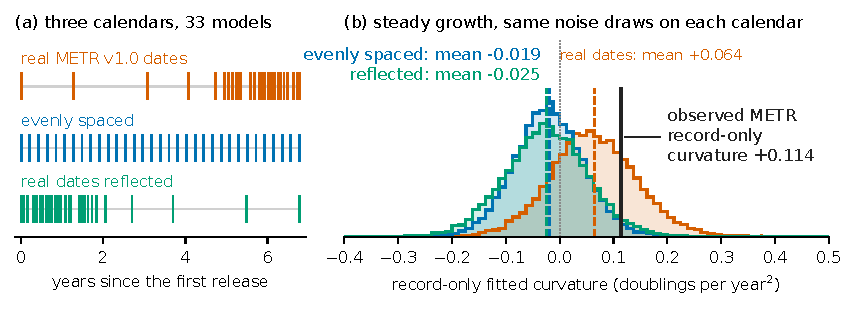
\includegraphics[width=0.74\textwidth]{figs/fig_open.pdf}
\caption{The sign of the selection effect depends on the release calendar. (a) Three calendars for \nModels\ models over the same span: the real METR version 1.0 release dates; evenly spaced dates; the real dates reflected. (b) Curvature of a quadratic fitted to the record-setting models only, over 20{,}000 data sets with exactly steady growth: a line at the simulator's null rate plus independent normal noise with the calibrated model-level standard deviation, the same draws on all three calendars. Dashed lines: the stored means (\schedRealBeta, \schedEvenBeta\ and \schedReflBeta; 40{,}000 data sets each). Solid line: the record-only curvature of the real series, \realSotaBeta, which is tested against a null fitted to the real series (Sec.~\ref{sec:real}).}
\label{fig:open}
\end{figure*}

\emph{What is new.} We measure how much fitting only record-setting models bends a benchmark trend, how the release calendar changes the sign of that bias, and how often tests of acceleration give false alarms or detect a real speedup. The closest work answers different questions. Kwa \emph{et al.}\ \cite{kwa2025} built the METR series and reported its trend, and METR has noted selection and measurement concerns about reading acceleration from it \cite{metr2026limits}, but neither source measures how selecting the records changes the fitted shape or gives a test of acceleration with a known false-alarm rate. Denain and Barry \cite{denain2026} compare candidate trend families by how well they predict later results; that is a forecast comparison, not a test with a stated false-alarm rate. Nguyen and Fithian \cite{nguyen2026} re-examine how each model's horizon is estimated from its task results; that concerns the height of each point, whereas our question is which points enter the trend, and it would remain if every horizon were estimated perfectly. Smith \cite{smith1988} fitted trends to annual athletics records by a likelihood that treats every non-record year as censored at the standing record; such estimators are sensitive to the assumed error distribution \cite{feuerverger1996}, and the finite-sample size and power of its test for a bend with a few dozen models had not, as far as we can find, been evaluated. We evaluate it here (Sec.~\ref{sec:size}). We use simulations with known growth rates to see what happens when the trend is fitted only to records.

None of the ingredients is ours. The statistics of records is classical \cite{arnold1998}, including records from sequences with a trend \cite{ballerini1985,ballerini1987b,franke2010,wergen2013,wiuff2026}, tests of trend from the number and timing of records \cite{foster1954,cebrian2021}, and the bias that selection on the outcome causes in regression \cite{heckman1979}. The closest analysis of acceleration in AI, that of Denain and Barry \cite{denain2026}, compares eight curve families by predictive accuracy, by default on the models that were state of the art on release, with a score-independent roster among the robustness checks; nothing here shows it wrong. We found no earlier statement that record-only sampling by itself produces curvature in a capability trend; this is not a claim of priority.

The plans, bars and reading rules were committed before the runs they govern, in stages, and several bars failed; the frozen texts, code and stored results are archived (\url{https://doi.org/10.5281/zenodo.24521481}). Most results were fixed in a later stage, after earlier results were known, and are exploratory in that sense; \SM\ Sec.~S1 and Table~S1 label each one. \textbf{Nothing in this paper is a confirmatory result about real AI progress.}

\section{Setting and methods}\label{sec:methods}
\emph{Data.} We use the public METR run-level file for the time-horizon analysis, version 1.0 (pinned by checksum, \runsSha), restricted to the \nModels\ models released up to 30 November 2025: 170 tasks in 50 task families. For each model we refit a ridge-penalised logistic regression of success on $\log_2$ of the human task time and take $y_m=\log_2$ of the time at which the fitted success probability is 50\%. A \emph{record} is a model whose $y$ strictly exceeds that of every earlier model; models released on the same day were processed in name order for every headline result. The sample has \nRecords\ records and \nNonRecords\ other models over \spanYears\ years. Three pairs of models share a release date, and reversing the within-day order changes the observed record count from \tieNameN\ to \tieRevN; taking only the best model per day moves the equivalent ratio of the reference simulation (defined below) from \tieRrName\ to \tieRrGroup\ (\SM\ Sec.~S5).

\emph{Curvature.} With $t$ the release date in years, we fit $y=b_0+b_1(t-\bar t)+\beta_2(t-\bar t)^2$ and call $\beta_2$ (doublings per year$^2$) the curvature. Steady exponential progress is $\beta_2=0$ and acceleration is $\beta_2>0$. To give a curvature a calendar meaning we quote the equivalent ratio $\rreq$: the growth rate at the end of the window divided by the rate at its start, for a quadratic trend with that curvature. It is $\rreq=(1+q)/(1-q)$ with $q=\beta_2\times\text{span}/\text{rate}$, where the rate is the growth rate at the middle of the window, \rateNull\ doublings per year in the simulator and \linSlope\ for the observed series (\SM\ Sec.~S1); for example $\hat\beta_2=\betaAll$ gives $\rreq=\rrEqAll$. Before the simulations that use it we fixed $\rr=2$ as the smallest acceleration we would call meaningful: a doubling time of \dblStartRrTwo\ days at the start of the window falling to \dblEndRrTwo\ at its end.

\emph{Simulator.} Each simulated data set keeps the real release dates and the real task, family and run structure. Model horizons follow an exact exponential, or a quadratic alternative indexed by $\rr$, plus an independent model-level offset with standard deviation \sigmaM\ ($\log_2$ units); task difficulty carries a jitter shared across models; run outcomes are binomial; and every horizon is re-estimated exactly as for the real data. The noise parameters were calibrated to the real data (\SM\ Table~S2). Eight variants change one feature at a time (evenly spaced dates, a lower suite ceiling, less model-level noise, a model-by-family interaction); with the real design they make nine \emph{null families}; the five that Table~\ref{tab:main} calls ``all five'' are the real design, even dates, a lower ceiling, halved model noise and a model-by-family interaction.

\emph{Tests.} We scored three kinds of procedure. The first fits the quadratic to the records only and tests it by the usual $F$ test or by a bootstrap. The second tries to correct the record fit: Smith's censored likelihood; the \emph{inverse-Mills} correction for the expected excess of each record, the device of Heckman \cite{heckman1979}; and a \emph{random audit}, which keeps every record and a random 25\% of the other models with weight 4 \cite{horvitz1952}. The third fits the quadratic to all models and uses the classical $t$ test, the heteroskedasticity-robust HC3 $t$ \cite{mackinnon1985}, or a wild bootstrap \cite{wu1986,davidson2008}. \emph{Record timing}, the mean record date minus the mean date of all models, is a diagnostic that uses no heights. Definitions are in \SM\ Secs.~S1 and S4.

A test is run upward at a one-sided 5\% and two-sided at 5\%. Its \emph{size}, the rejection rate when progress is exactly steady, is called acceptable in a cell if the Clopper--Pearson (CP) \cite{clopper1934} 95\% interval of that rate lies inside a band fixed in advance, $[3.5\%,6.5\%]$. \emph{Size-adjusted power} replaces the nominal cut-off by the empirical 5\% cut-off from an independent null cell; such a cut-off is known only inside a simulator, so for a test that misses its nominal size this power cannot be had in practice.

\section{Results}\label{sec:res}

\subsection{Record selection bends the fitted trend}\label{sec:bias}
Under exactly steady progress in the reference simulation, the mean curvature of the record-only fit is \biasSota\ doublings per year$^2$ (standard error \biasSeSota), against \biasAll\ for the fit through all models (\SM\ Table~S9). The equivalent ratio is $\rreq=\biasRrSota$: on average the record-only fit bends upward as much as a trend whose growth rate rises by that factor across the window.

The reason is simple. A model becomes a record only if it beats all its predecessors, which requires more favourable noise the more recent competitors there are, and on the METR calendar releases are sparse early (three models in four years) and dense late. Selection on independent noise is enough to produce the effect. With independent Gaussian horizons at the real dates and nothing else, the all-model curvature is unbiased (mean \ladZeroAll, SE \ladZeroSe) and the record-only fit already has $\rreq=\ladZeroRecRr$; adding horizon estimation, the suite ceiling, shared task jitter and a model-by-family interaction moves that figure only between \ladRecRrMin\ and \ladRecRrMax\ (\SM\ Table~S5).

The direction is not general. With the noise, span, rate and number of models held fixed (\cfReps\ data sets per schedule; \SM\ Table~S17), the mean record-only curvature was above zero at the real dates ($\rreq=\cfRealRr$), below zero in \cfNeg\ of the \cfOther\ other schedules, among them even spacing (\cfEvenRr), the real dates reflected (\cfReflRr) and two smooth schedules that grow denser late, and indistinguishable from zero in one. Denser late releases are therefore not sufficient, and we have not isolated which feature of a schedule sets the sign; a closed-form approximation specified in advance failed its tolerance (\SM\ Sec.~S6). The effect should be simulated for the calendar at hand.

Other benchmarks show the same thing. We took every public benchmark file of Epoch AI \cite{epochdata} with at least 30 models, 8 records and 15 distinct release months: \mbN\ series of \mbMmin\ to \mbMmax\ models. Scores lie between 0 and 1 and were analysed on the logit scale, with each series truncated before the first record reaching 90\% of its ceiling. In each series we permuted the release dates among the models 1000 times, which removes any relation between score and date while the record rule still selects, and then planted a known trend (half a standard deviation of the logit scores across the span) and an upward bend (a further half standard deviation at the end of the span). The plan committed before the audit ran registered these planted runs: the bootstrap's size with the planted trend, and its pooled coverage and bias for the planted bend, are confirmatory bars (\SM\ Table~S1). The sign count by series that follows is a descriptive summary that no bar fixed. The mean fitted record curvature had the opposite sign to the planted bend in \mbBiasNegSign\ of the \mbN\ series (\SM\ Table~S7). This suggests that on such calendars selection could hide a real acceleration; that is an inference from the sign of the bias, and we did not simulate it in the METR design.

The bias can be reduced when the models that did not set records are also observed. The inverse-Mills correction and the random audit brought the mean bias in the reference simulation down to $\rreq=\biasRrHeck$ and \biasRrAudit. Both use non-record models, so neither helps a reader who has only the records.

\subsection{Tests of acceleration: false alarms and low power}\label{sec:size}\label{sec:power}
\emph{Tests on the records.} On \origIidN\ data sets with exactly steady progress, the usual $F$ test on the quadratic term of the record-only fit rejected, two-sided, in \origIid\% (CP 95\% interval \origIidLo--\origIidHi\%) at a nominal 5\%. A bootstrap over task families, tasks and runs, which we had expected to repair this, rejected in \origHb\% (\origHbLo--\origHbHi\%): resampling tasks and runs leaves out the model-level scatter, which is the larger part of the noise. A bootstrap that resamples models has a two-sided rate near nominal at the real design (\aTwoMbSotaTwoX\%); its separate one-sided 5\% tests reject at \aTwoMbSotaUpX\% upward and \aTwoMbSotaDnX\% downward, so its rejections are almost all upward, which is what a bias produces. In the \mbN\ benchmark series with permuted dates and no planted trend, the two-sided $F$ test on the record points was oversized (above 10\%, CP lower limit above 7\%) in \mbBarOne\ of \mbN\ series, counting only permutations in which the fit is defined (the 90\% truncation is applied once to the original series and the dates are then permuted within that fixed sample, so a permutation can leave too few records for the quadratic to be fitted), and in \mbIidTwoOverAtt\ with undefined fits counted as non-rejections; the upward one-sided version was oversized in \mbIidOneOver\ series. Smith's censored-likelihood test of curvature rejected a true steady trend in \sizeCclUp\% of simulated data sets at a nominal 5\%, and with a cut-off calibrated inside the simulator it detected a doubling of the growth rate in \powMaxTwo\% (below). The model-level bootstrap did not generalise either: it was oversized in \mbOver\ series, and its intervals covered a planted upward curvature in \mbCovPlus\ of replicates (nominal 0.95; \SM\ Sec.~S7).

\emph{Corrected tests.} Reducing the bias in the mean does not make a test honest (Table~\ref{tab:main}). The inverse-Mills, random-audit and record-timing statistics are referred to the same all-model parametric-bootstrap null as the record-only fit, with the baseline line and residual standard deviation estimated from all models. Of the \nMethods\ corrections and diagnostics scored, \nSizeValid\ had acceptable size at the real design, the random audit and record timing among them; the two likelihood tests, referred to their asymptotic normal distribution, were far outside the band (\sizeCclUp\% and \sizeTclUp\% upward). Only \nRobust, record timing and two other diagnostics, stayed inside the band in all five null families in which they were run; the random audit became oversized when the model-level noise was halved (\SM\ Tables~S3, S8).

\emph{Tests on all models} need no correction for selection. At the real design HC3 is within the band (\aTwoHcUp\% upward, CP \aTwoHcUpLo--\aTwoHcUpHi\%; \aTwoHcTwo\% two-sided), as is the wild bootstrap (\aTwoWildUp\% and \aTwoWildTwo\%); the classical $t$ test is oversized (\aTwoOlsUp\%, \aTwoOlsTwo\%). This is not a general licence: for HC3 and the wild bootstrap the verdict holds in four of the eight other null families and fails in the other four (\SM\ Table~S8), and none of the families includes dependence among models from one developer.

\emph{Power} (10{,}000 replicates per alternative; \SM\ Table~S4). Among the eleven record-based procedures with reported size-adjusted power, the maximum at $\rr=2$ was \powMaxTwo\%, for the censored likelihood, which itself misses nominal size; the random audit and record timing reach \powAuditTwo\% and \powRrateTwo\%. None reaches 80\% even at $\rr=4$ (largest \powMaxFour\%). The HC3 test has a size-adjusted power of \aTwoPowHcTwo\% at $\rr=2$ (95\% interval \aTwoPowHcTwoLo--\aTwoPowHcTwoHi\%) and \aTwoPowHcFour\% at $\rr=4$. That figure is for the HC3 statistic with a cut-off calibrated in the simulator; the wild bootstrap uses the same statistic, so its size-adjusted entry is the same rule and adds nothing. Used as a test in its own right, at its nominal 5\% cut-off, the wild bootstrap has a power of \aTwoRawWildTwo\% at $\rr=2$. A failure to detect acceleration with \nModels\ models therefore does not rule out a doubling of the growth rate. Low power also inflates what does pass: among replicates at $\rr=2$ in which the audit test rejected, the mean curvature estimate was \typeMAuditTwo\ times the true curvature for the audit fit and \typeMAllTwo\ times for the all-model fit \cite{gelman2014} (\SM\ Table~S10).

\begin{table*}[t]
\caption{Key procedures at the real design (\SM\ Tables~S3, S4, S8 give all procedures and null families). Size: rejection rates (\%) under an exactly exponential trend at a nominal 5\%, 40{,}000 replicates; ``up'' upward 5\%, ``two'' two-sided 5\%; unmarked: within the band $[3.5,6.5]\%$; $\dagger$ inconclusive; $\ddagger$ outside. The record-only fit is tested against the parametric-bootstrap null (a line fitted to all models plus independent normal noise); the naive $F$ test and the record model bootstrap are not shown (not size-valid). ``Size-valid'': both rates within the band at the real design; ``all five'': within the band in every one of five null families. Power: size-adjusted power (\%) at $\rr=2$ and $\rr=4$ (10{,}000 replicates), and raw power at $\rr=2$ with the nominal cut-off.}
\label{tab:main}
\begin{ruledtabular}
\begin{tabular}{lccccccc}
 & \multicolumn{4}{c}{size} & \multicolumn{3}{c}{power, $\rr$} \\
Procedure & up & two & size-valid & all five & 2 & 4 & raw, 2 \\
\hline
record-only fit, parametric bootstrap & 5.9 & 6.6$^{\dagger}$ & no & no & 17.9 & 38.3 & 21.6 \\
censored likelihood & 11.8$^{\ddagger}$ & 12.2$^{\ddagger}$ & no & no & 27.9 & 61.4 & 46.4 \\
inverse-Mills & 6.6$^{\dagger}$ & 6.4$^{\dagger}$ & no & no & 19.4 & 41.9 & 25.2 \\
random audit & 6.0 & 6.2 & yes & no & 24.5 & 52.8 & 27.5 \\
record timing & 4.7 & 4.5 & yes & yes & 13.4 & 27.0 & 13.2 \\
HC3 $t$, all models & 5.1 & 5.1 & yes & no & 34.0 & 68.5 & 34.7 \\
wild bootstrap, all models & 4.8 & 4.6 & yes & no & 34.0 & 68.5 & 33.0 \\

\end{tabular}
\end{ruledtabular}
\end{table*}

\subsection{The observed METR series}\label{sec:real}
\begin{figure}[t]
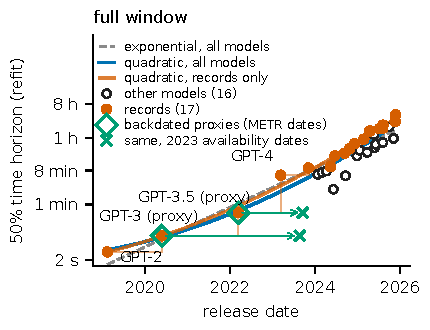
\includegraphics[width=\columnwidth]{figs/fig_real.pdf}
\caption{The real series: our refit of the 50\% time horizon for the \nModels\ models of the METR time-horizon data (version 1.0) released to November 2025. Filled: the \nRecords\ record-setting models, joined by the best-so-far step line; open: the other models. Dashed: exponential fit to all models (doubling time \linDbl\ days). Blue: quadratic fit to all models. Orange: quadratic fit to the records only. Green diamonds: the two backdated proxy models (davinci-002, gpt-3.5-turbo-instruct) at the dates METR gives them; crosses: the same models at their 2023 availability dates. Under no acceleration the record-only curvature has a null mean of \realSotaNull, not zero.}
\label{fig:real}
\end{figure}

We applied these tools to the real series once, under a plan and a reading rule committed beforehand (commit \preregReal; \SM\ Sec.~S5). The series had already been examined, there is a single benchmark, and the deciding tests treat the models as independent, so what follows is exploratory (Fig.~\ref{fig:real}; \SM\ Table~S11).

\emph{The record curve.} The record-only curvature is \realSotaBeta, against a mean of \realSotaNull\ under steady growth ($p_{\rm up}=\realSotaPup$). The bend of the best-so-far curve is therefore compatible with constant growth. That does not show how much of the bend selection caused, or that there is no acceleration.

\emph{All models.} The all-model fit has positive curvature (\betaAll\ doublings per year$^2$, HC3 95\% interval $[\hcCiLo,\hcCiHi]$; HC3 $p_{\rm up}=\hcPup$, Holm-adjusted \cite{holm1979} over the six planned statistics \holmHc), and the random-audit test agrees ($p_{\rm up}=\realAuditPup$). Our rule, fixed in advance, permitted the words ``evidence of acceleration'' when both the HC3 and the random-audit one-sided $p$-values were below 0.05 and the Holm-adjusted HC3 value was below 0.10; all three held. The fixed audit draw exceeded \auditManyShare\% of \auditManyN\ further redraws, so the audit test depends on which random subsample is drawn. We do not adopt those words, because the evidence that the curvature is more than chance does not survive four reasonable changes.

The first is dependence within developers. The \nModels\ models come from \clG\ developers; one supplies \clMax\ and another \clSecond. Allowing errors to be correlated within a developer, a cluster-robust $t$ test \cite{bell2002,imbens2016} gives $p_{\rm up}=\clP$, a wild cluster bootstrap \cite{cameron2008,webb2023} \clWebb, and exact enumeration of the \clRadN\ sign patterns \clRad. None is below 0.05, though with \clG\ clusters the power of such tests is presumably low, and no developer-clustered test met the prespecified size criterion in all six calibration cells (\SM\ Sec.~S5, Table~S16).

The second is the two earliest models. Leaving out one model at a time keeps the HC3 $p_{\rm up}$ below 0.05 for \looNsig\ of the \nModels\ models; the exceptions are GPT-2 ($p_{\rm up}=\looPGptTwo$) and GPT-3 (\looPGptThree). Without both, the curvature rises from \betaAll\ to \dropFirstTwoBeta\ while $p_{\rm up}$ rises to \dropFirstTwoP: those models supply the precision, not the sign. OpenAI's models hold \levOpenAI\% of the leverage on the squared-date term, and without them $p_{\rm up}=\looOpenAIP$ (\SM\ Tables~S12, S14).

The third is that these early anchors are also the least comparable measurements. GPT-2's horizon rests in part on \impN\ imputed zero scores \cite{kwa2025}; without them $p_{\rm up}=\impP$. Two models, davinci-002 and gpt-3.5-turbo-instruct, carry the release dates of GPT-3 (2020) and GPT-3.5 (2022), for which they stand in \cite{kwa2025}, although both became available in 2023 \cite{metr2026risk}. With their 2023 availability dates $p_{\rm up}=\proxAvailP$, with one alternative dating \proxAvailPb, and without the two models \proxDropP\ (\SM\ Table~S13). METR also reports that a penalty in its horizon model, since removed, lowered the horizons of weak models and raised those of strong ones \cite{metr2026modelling}; our ridge penalty has not been checked for that effect.

The fourth is a rival explanation. A fixed September 2024 break (the release of o1-preview) allowing a jump in level and a change of slope fits about as well as the quadratic on AICc, BIC and leave-one-month-out error, and absorbs the curvature (developer-clustered two-sided $p=\hgCQHp$ for the quadratic term with the break in the model). A one-time step and a steady acceleration call for different forecasts. The positive control for the quadratic in that comparison missed its bar, so we give no formal verdict on whether these data can separate the two (\SM\ Sec.~S5, Table~S15). Denain and Barry's related fit groups models by reasoning status \cite{denain2026}.

Two further checks do not change this picture. Records fall later in the window than a steady trend with this noise predicts (record timing \realRrateObs\ years against a null mean of \realRrateNull; $p_{\rm up}=\realRratePup$, Holm-adjusted \holmRrate), but that diagnostic assumes independent models and also responds to falling noise. A replication on METR's version 1.1 runs \cite{metr2026th11}, which selects the records on one half of the tasks and refits them on the other, detected no shrinkage of the record curvature (difference \stDone; 95\% interval \stDoneLo\ to \stDoneHi), an interval wide enough to contain the whole simulated selection bias. Finally, the all-model curvature converts to $\rreq=\rrEqAll$, which is not a usable estimate: one that passes a significance gate at this power is expected to be too large.

\section{Limits and practice}\label{sec:disc}
The simulations rest on one series and one calibrated simulator with eight variations, which models dependence through shared tasks but not through developers, and the null used for several tests assumes independent normal residuals of constant variance about a line. What is estimated is the curvature of our refitted horizons on a fixed suite, and the horizon-fitting model itself can matter \cite{nguyen2026}. Fitting all models is not a cure for selection in general. Labs choose what to release and when, and evaluators choose which non-frontier models to run; if that choice changes over time (more small or open-weight models late in the window, or only flagships early), the all-model quadratic can be biased in either direction. We did not model this, so the all-model estimate is conditional on the observed roster. The quadratic is one alternative among many (the break was tried at one date), the size band is of our own choosing, and the benchmark audit covers two record-series tests, conditional on a defined fit. We did not simulate the joint reading rule or take a confirmatory step on unseen models.

For practice we suggest four habits. Report and plot all evaluated models alongside the records, and say how the non-frontier models were chosen. Check a bend in a best-so-far curve, in either direction, against a null simulated for the actual release schedule. Check sensitivity to within-developer dependence, noting that with few developers cluster-robust tests have low power. And report a failure to detect acceleration together with the power of the test.

\section{Provenance, assistance and author statement}
We used blueMonster, a tool developed by MOBLUEHQ, Inc., to generate research topics and brainstorm ideas. Candidate correction methods and the closed-form approximation were suggested by a second internal brainstorming aid; each was implemented and judged by the simulations reported here. The simulation code, the pre-registered plans, the analysis and this draft were written with Claude large language models (Anthropic) under the author's direction. Two further large language models (ChatGPT, OpenAI; Gemini, Google) criticised the results and earlier drafts, and several analyses and corrections follow from their comments. These were AI-assisted critiques, not peer review, and no human referee has read this draft. The numbers in the text and tables are written by a script from the committed result files, with a manifest giving the source of each, and the figures are drawn from the same files. The author takes responsibility for the content.

The author is an amateur. He has no formal training in statistics, econometrics or machine-learning evaluation and has published no research in them. Much of this work was done while improving MOBLUEHQ's software tools, by using them on a real problem, and in order to learn how such research is done. His inexperience should invite heavy scepticism towards the methods and the claims: errors of a kind a trained researcher would not make are possible, and the checks described here lower that risk without removing it. He welcomes corrections.

\emph{Competing interests.} The author is the founder of MOBLUEHQ, Inc., which develops and intends to sell blueMonster.

\section*{Data and code availability}
The METR run-level data are public (METR, \texttt{eval-analysis-public} repository), as are the Epoch AI benchmark files (CC BY 4.0); both are pinned by checksum (\SM\ Sec.~S8). The frozen pre-registration texts and the manifest tying each number here to its source file accompany the preprint. The archive (code, stored results, pre-registration texts and a one-command regeneration of its numbers) is public at \url{https://github.com/mobluehq-llc/record-selection-frontier-curvature} and is archived at Zenodo, \url{https://doi.org/10.5281/zenodo.24521481} (release v1.0). That release regenerates the numbers of draft v10; the scripts updated since, which regenerate every number in this version, will be archived in the next Zenodo release.

\bibliography{refs}

\end{document}
